%%%%%%%%%%%%%%%%%%%%%%%%%%%%% Define Article %%%%%%%%%%%%%%%%%%%%%%%%%%%%%%%%%%
\documentclass{article}
%%%%%%%%%%%%%%%%%%%%%%%%%%%%%%%%%%%%%%%%%%%%%%%%%%%%%%%%%%%%%%%%%%%%%%%%%%%%%%%

%%%%%%%%%%%%%%%%%%%%%%%%%%%%% Using Packages %%%%%%%%%%%%%%%%%%%%%%%%%%%%%%%%%%
\usepackage{listings, xcolor}
\usepackage{parskip}
\usepackage{hyperref}
\usepackage{amsmath}
\usepackage{graphicx}
\usepackage[a4paper, margin = 1.5cm]{geometry}
\usepackage{float}
\usepackage{amsmath}
\usepackage{amssymb}
\usepackage{parskip}
\usepackage{listings}

\lstset{
frame = shadowbox,
basicstyle = \small\ttfamily,
mathescape = true,
numbers = left,
commentstyle = \itshape\color{gray}
columns = flexible,
keepspaces = true,
moredelim = [l]{//}
}

%%%%%%%%%%%%%%%%%%%%%%%%%%%%%% Title & Author %%%%%%%%%%%%%%%%%%%%%%%%%%%%%%%%
\title{Activity Diagram}
\author{Trentin Tommaso}
%%%%%%%%%%%%%%%%%%%%%%%%%%%%%%%%%%%%%%%%%%%%%%%%%%%%%%%%%%%%%%%%%%%%%%%%%%%%%%
\begin{document}
  \maketitle
  \tableofcontents
  \newpage
  
  \section{Notazioni}
    \subsection{Diagrammi di attività}
      Estensione di diagrammi di flusso che introduce esecuzioni concorrenti e permette di modellare logica procedurale di un algoritmo ma anche processi di business / workflow esistenti nella realtà da modellare.
    \subsection{Attività / Azioni}
      \begin{itemize}
        \item \textbf{Attività} corrisponde a insiseme coerente di azioni elaborative compiute dal sistema;
        \item \textbf{Azione} èun'unità di lavoro atomica all'interno dell'attività, un AD rappresenta una singola attività composta da azioni.
      \end{itemize}
    \subsection{Flussi}
      \begin{itemize}
        \item Modellato mediante frecce entranti / uscenti che collegano le attività, per convenzione ingresso coincide con inizio e uscita con completamento dell'operazione; 
        \item Nodi iniziali e finali indicano inizio e fine dell'elaborazione;
        \item Se esistono più nodi iniziali di un'attività, i flussi cominciano simultaneamente e vengono eseguiti in parallelo. 
      \end{itemize}
      \begin{figure}[htpb]
          \centering
          
\includegraphics[width=0.5\linewidth]{figures/flu.png}
      \end{figure}
    \subsection{Branch}
      \begin{itemize}
          \item Azione di decisione, corrisponde ad un IF con un arco entrante e più archi uscenti; 
          \item Ciascun arco etichettato con condizione booleana (condizioni devono esssere mutualmente esclusive); 
          \item Dopo una decisione si deve intraprendere uno solo dei flussi uscenti.
      \end{itemize}
      \begin{figure}[htpb]
          \centering
          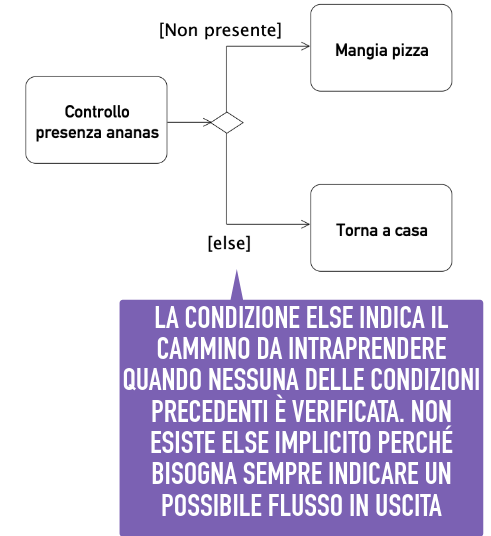
\includegraphics[width=0.35\linewidth]{figures/fl_br.png}
      \end{figure}
    \subsection{Merge}
      Segnala fine del comportamento condizionale iniziato da una \textbf{branch}, ha più archi entranti e uno uscente.
      \begin{figure}[htpb]
          \centering
          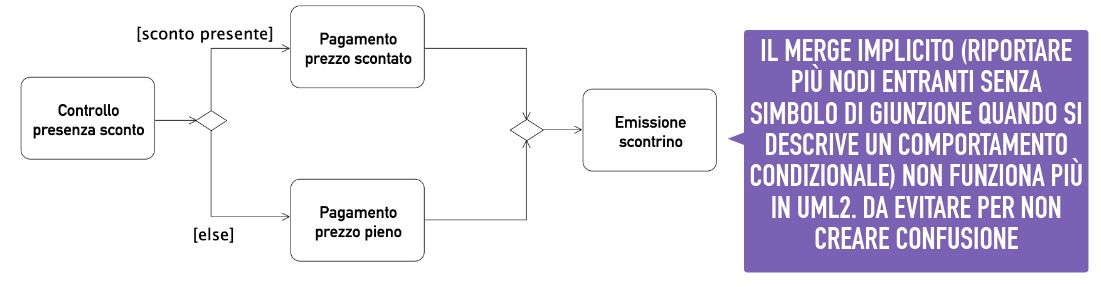
\includegraphics[width=0.5\linewidth]{figures/fl_me.png}
      \end{figure}
    \subsection{Fork / Join}
      \noindent
      \begin{minipage}[c]{0.68\linewidth}
          \begin{itemize}
              \item \textbf{Fork} rappresenta biforcazione del flusso tra 2+ thread (un arco entrante e più uscenti, rappresentanti thread paralleli eseguiti concorrentemente); 
              \item \textbf{Join} è duale del fork, sincronizza più flussi concorrenti (più archi entranti e uno uscente).
              \item Presenza di un \textit{fork} indica che l'ordine di esecuzione tra i flussi non è rilevante (possono anche avvenire in parallelo); 
              \item Presena di \textit{join} indica che attività successiva può essere eseguita \textbf{solo} quando tutti i flussi in entrata sono terminati (altrimenti eseguita appena arriva il primo dei flussi di entrata).
          \end{itemize}
      \end{minipage}
      \hfill
      \begin{minipage}[c]{0.28\linewidth}
          \centering
          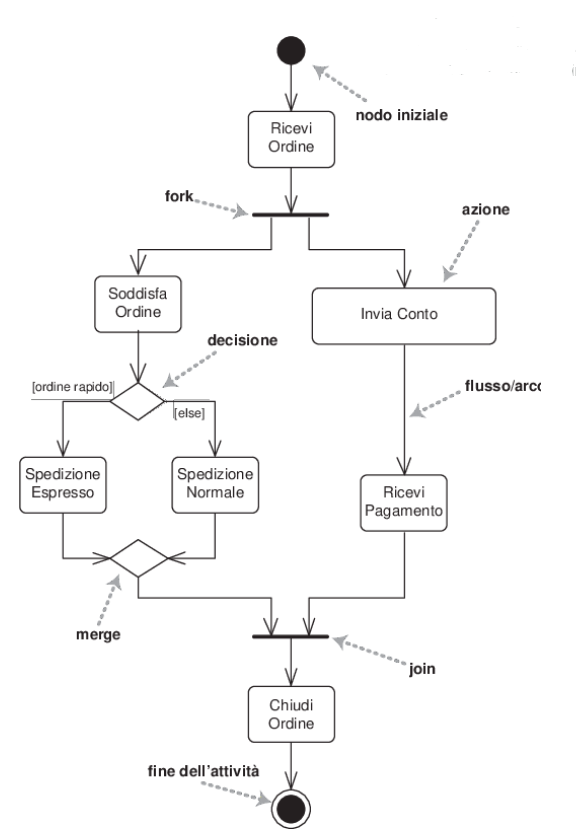
\includegraphics[width=\linewidth]{figures/fl_fo_jo_2.png}
      \end{minipage}
      \subsubsection{Esempi}
        \begin{figure}[htpb]
          \centering
          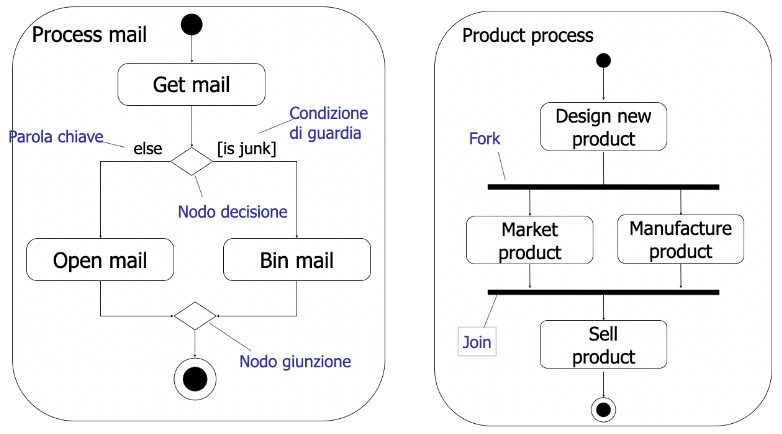
\includegraphics[width=0.8\linewidth]{figures/fl_es.png}
        \end{figure}
  \section{Scomposizione di un'azione}
    Nella notazione precedente non è rappresentato quale parte del SW è responsabile di determinate azioni, inoltre in caso di attività complesse il diagramma è difficile da leggere.
    \subsection{Macroattività / Sottoattività}
      \begin{itemize}
          \item Per supportare diversi livelli di astrazione si possono racchiudere porzioni di un'attività complessa in macroattività; 
          \item Le azioni delle macroattività vengono dettagliate in grafici separati; 
          \item Macroattività vengono indicate con simbolo del rastrello all'interno del rettangolo.
      \end{itemize}
      \begin{figure}[htpb]
          \centering
          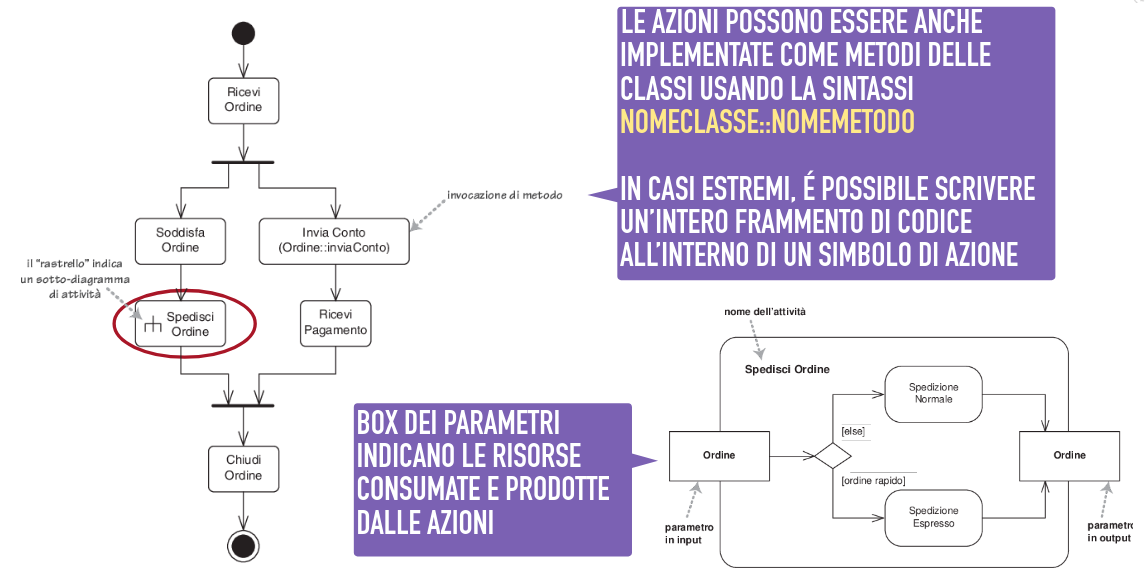
\includegraphics[width=0.8\linewidth]{figures/macro.png}
      \end{figure}
\end{document}
